%% EXERCICIOS PARA INCLUÍR DENTRO DO CADERNO DE EXERCICIOS %%
%
% EXERCICIO.- COMENTARIO AUDICIÓN PUER NATUS EST NOBIS
%
\section{Monodia profana: comentarios de audición} \label{sec:modelo-trovadorescas}
%
Cando realizamos un comentario de audición dunha canción trobadoresca ou trobeira, teremos en conta na análise da mesma os aspectos seguintes: modo, estilo de canto, ámbito melódico e por último a estrutura formal da obra.

\begin{multicols}{2}
    \begin{enumerate}[a)]
\item \textbf{Modo}.
No caso das cancións trobadorescas e trobeiras --e en xeral na monodia profana-- utilizamos os nomes de orixe grego da teoría musical: dórico, frixio, lidio e mixolidio. Os nomes eclesiásticos (\textit{protus, deuterus, tritus} e \textit{tetrardus}) igual que os números de modo empregarémolos no canto litúrxico.

\item \textbf{Estilo de canto}.
Diferenciamos dous estilos básicos: <<silábico>> e <<ornamentado>>. Estas cancións non teñen un estilo único, oscilando ás veces entre ambos; indicaremos o que predomina dos dous e igualmente, as diferencias entre versos e seccións.

\item \textbf{Ámbito melódico}.
Para coñecer o ámbito melódico, terase en conta o intervalo entre a nota máis grave e a máis agruda, e a distancia entre ámbalas dúas e a nota final. Tamén se indican as diferenzas de ámbito entre seccións ou versos da canción.

\item \textbf{Estrutura formal}.
Se partimos da obra con texto completao, indicaremos o número total de estrofas, e a presencia da <<tornada>>.
Na estrofa, debemos examinar a liña melódica de cada verso elaborando un esquema; asignaremos letras a diferentes melodías. Se a estrofa se divide en seccións, tamén se indica.
    \end{enumerate}
\end{multicols}
%
\subsection*{Exemplo de comentario: \textit{A chantar m’er de so qu’ieu non volria}} 
A audición proposta como exemplo de comentario, corresponde a unha canción monódica de estilo trobadoresco, da condesa Beartix de Dia. 
\\ 
(Enlace: \href{https://hesperetusa.wordpress.com/2011/04/22/a-chantar-mer-de-so-quieu-non-volria/}{Hesperetusa})

\begin{multicols}{2}
%\begin{enumerate}[1.-]
%PUNTO NÚMERO 1: ESCOITAR A PEZA
%
\subsubsection*{Paso no. 1: análise da partitura} 

No caso de dispoñer de copia impresa da obra, o primeiro que debemos realizar é unha vista previa da mesma tratando de identificar aqueles elementos descoñecidos e que polo tanto será preciso descifrar antes de proceder.

\subsubsection*{Paso no. 2: escoita activa} 

Despois da observación e lectura e identificaremos os elementos formais por medio dunha escoita activa da obra.
É moi importante identificar auditivamente todo o que observamos no paso 1.
A escoita activa, axudaranos a determinar a relación música-texto da obra neste caso.

\subsubsection*{Paso no.3: datos da audición} 

Unha vez realizados os pasos 1 e 2 prestaremos atención aos seguintes puntos.
%
    \begin{enumerate}[1.-]
% ANÁLISE DO RITMO DA OBRA:
        \item % RITMO
        \textbf{Ritmo}. Identificamos o ritmo, tendo en conta: pulso, indicacións de compás e outras indicacións dinámicas. 
        Neste caso, estamos ante un ritmo:
        \begin{enumerate}[a)]
            \item mensural 
            \item non mensural 
        \end{enumerate}
% ANÁLISE DA MELODÍA DA OBRA:
        \item %MELODÍA:
        \textbf{Melodía}. Tendo en conta a melodía, determinamos o modo, ámbito e estilo. Prestaremos atención ao perfil melódico e interválica, observando se hai grandes saltos ou mais ben discorre por graos conxuntos.
%        \begin{multicols}{2}
        \begin{enumerate}[a)]
            \item 
            Que intervalos se repiten con maior frecuencia? \dotfill
            \item 
            Cal é o maior intervalo que podemos atopar na peza? \dotfill
            \item
            Podemos afirmar que a melodía se move por graos \dotfill
        \end{enumerate}
%        \end{multicols}
        Vexamos a continuación o Modo, Ámbito e Estilo tendo en conta a melodía:
        \begin{itemize}
% ANÁLISE DO MODO:
            \item % MODO
            \textbf{Modo}.
        \begin{itemize}            
            \item 
            Identifica a clave \dotfill
            \item 
            Cal é a nota \textit{finalis}? \dotfill
            \item
            En que modo básico estamos? \dotfill
            \item
            Cal é a nota máis agura? \dotfill 
            \item
            Cal é a nota máis grave? \dotfill 
            \item
            Que intervalo forma coa final? \dotfill
            \item
            Cal é a nota tenor? \dotfill 
            \item
            En qué modo esta a obra? \dotfill
       \end{itemize}
% ANÁLISE DO ÁMBITO DA OBRA:
            \item % ÁMBITO
            \textbf{Ámbito}. \\
            Fixándonos na nota \textit{finalis} e na máis aguda:
                \begin{itemize}
                    \item
                    Que intervalo forman? \dotfill
                    \item
                    A melodía é de ámbito \dotfill
                \end{itemize}
            \item % ESTILO
            \textbf{Estilo do canto}. \\ Segundo a relación musica-texto, estamos ante un estilo:
                \begin{enumerate}[a)]
                  \item
                  Silábico \dotfill
                  \item
                  Neumático \dotfill
                  \item
                  Melismático \dotfill
                \end{enumerate}
        \end{itemize}
        \item % TIMBRE
        \textbf{Timbre}. \\
        Segundo as características da obra, debemos diferenciar as voces, instrumentos, formacións, agrupacións, ...
            \begin{itemize}
                \item 
                Que timbres recoñeces? \dotfill
                \item
                Polo tanto, trátase de \dotfill
            \end{itemize}
% ANÁLISE DA TEXTURA DA OBRA:
        \item %TEXTURA
        \textbf{Textura}. \\
        Polas características da obra, diferenciamos unha textura melódica \ldots 
            \begin{enumerate}[a)]
                \item 
                De escrita horizontal, monódica
                \item 
                De escrita horizontal, polifónica
            \end{enumerate}
% ANÁLISE DA FORMA DA OBRA
        \item %FORMA:
        \textbf{Forma}. \\
        Determinamos a forma segundo a extensión, textura e estrutura da obra. \\ 
        Convén lembrar aquí a seguinte clasificación:
            \begin{enumerate}[a)]
                \item
                Segundo a extensión:
                \begin{itemize}
                    \item
                    \textbf{Formas maiores}, de diferentes movementos ou grandes dimensións
                    \item
                    \textbf{Formas menores}, un só movemento ou de curta duración
                \end{itemize}
                \item
                Segundo os instrumentos ou voces:
                 \begin{itemize}
                    \item
                    \textbf{Formas vocais}, con intervención da voz humana
                    \item
                    \textbf{Formas instrumentais}, só instrumentos
                \end{itemize}
                \item 
                Segundo a súa estrutura:
                \begin{itemize}
                    \item 
                    \textbf{Formas estruturadas}, ou fixas: aquelas con esquema compositivo determinado
                    \item
                    \textbf{Formas libres}: non respetan aparentemente ningunha estrutura definida
                \end{itemize}
            \end{enumerate}
        \par %Pregunta sobre as Formas
        A que tipo de forma, podemos dicir que se axusta esta obra? 
        \begin{enumerate}[a)]
            \item 
            Forma vocal menor libre
            \item
            Forma vocal menor ternaria
            \item
            Forma vocal maior ternaria
            \item
            Forma instrumental menor ternaria
        \end{enumerate}
        \end{enumerate}
%    \end{multicols}
%
\end{multicols}
%\vspace*{0.25cm}
%
\subsubsection*{Paso no.4: clasificación} 
Unha vez realizada a análise da audición, tendo en conta os datos obtidos no paso 3, clasificaremos a obra tendo en conta sobre todo o ámbito e estilo.
%
% RESUMO DA AUDICIÓN DO EXERCICIO
%
\vspace*{0.25cm}
\begin{ejercicio}[Características principais da audición: «Puer natus est»]

% ESPACIO PARA REDACTAR O COMENTARIO DA AUDICIÓN
%
%\small{Trátase dunha forma vocal menor, de estrutura ternaria; segundo o ámbito e estilo, obedece a un canto antifonal do propio da misa cantado a capella por un coro de voces masculinas; a textura monódica horizontal é propia do canto chá (Gregoriano) en estilo neumático na primeira sección e silábico na segunda, de ámbito reducido escrita no modo \textit{tetrardus auténtico} (VII)     }

        \vspace*{2.78cm}
\end{ejercicio}

% ----------------------
% Partitura de audición:
% ----------------------
%\begin{figure}[h]
%    \centering
%    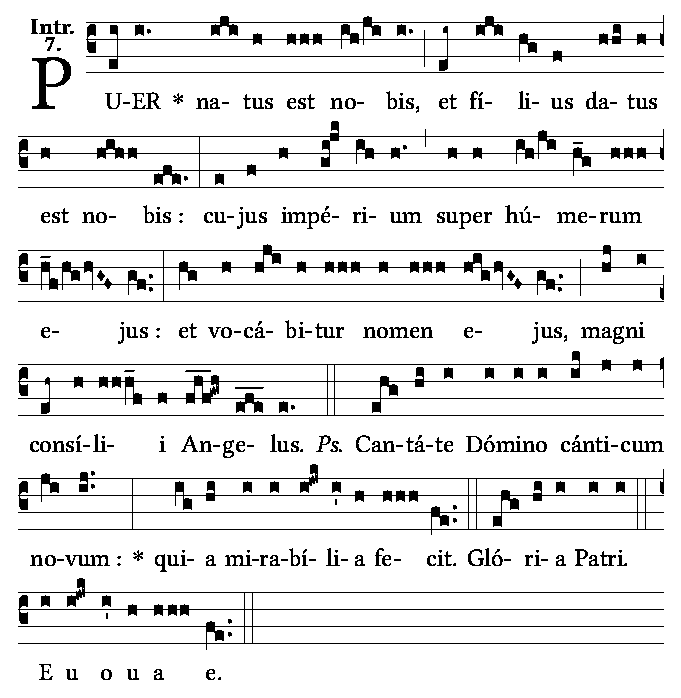
\includegraphics[width=0.75\textwidth]{figures/audicions/Puer-natus.eps}
%    \caption{Partitura do Introito «Puer natus est»}
%    \label{fig:puer-natus}
%\end{figure}
% -----------------------
%